\documentclass[oneside,english]{article}
\usepackage[T1]{fontenc}
\usepackage[utf8]{inputenc}
\usepackage{csquotes, caption}
\usepackage[colorlinks=true, citecolor = blue]{hyperref}      % hyperlinks
\usepackage{multirow, amssymb, amsmath, graphicx, arydshln, url, amsthm}
\usepackage[T1]{fontenc}
\usepackage{natbib}
\usepackage{babel}

\makeatletter
%%%%%%%%%%%%%%%%%%%%%%%%%%%%%% Textclass specific LaTeX commands.
\numberwithin{equation}{section}
\numberwithin{figure}{section}
\theoremstyle{plain}
\newtheorem{thm}{\protect\theoremname}
\theoremstyle{plain}
\newtheorem{lem}[thm]{\protect\lemmaname}

\makeatother

\usepackage{babel}
\providecommand{\lemmaname}{Lemma}
\providecommand{\theoremname}{Theorem}


\renewcommand\thefigure{\arabic{figure}}
\setcounter{figure}{0}

\makeatletter
\numberwithin{equation}{section}
\numberwithin{figure}{section}
\makeatother

\title{Supporting Information for ``Modelling publication bias and \textit{p}-hacking'' \\ by Jonas Moss and Riccardo De Bin}

\author{}

\date{}

\begin{document}

\maketitle

%% LyX 2.3.6.1 created this file.  For more info, see http://www.lyx.org/.
%% Do not edit unless you really know what you are doing.
\documentclass[oneside,english]{amsart}
\usepackage[T1]{fontenc}
\usepackage[latin9]{inputenc}
\usepackage{amsthm}

\makeatletter
%%%%%%%%%%%%%%%%%%%%%%%%%%%%%% Textclass specific LaTeX commands.
\numberwithin{equation}{section}
\numberwithin{figure}{section}

\makeatother

\usepackage{babel}
\begin{document}
\begin{proof}[(Rest of the) proof of Proposition 1]
For the random effects model, let us start from
\[
f(x_{i}\mid\theta_{0},\tau,\sigma_{i})\propto\sum_{j=1}^{J}\rho_{j}\int1_{[\alpha_{j-1},\alpha_{j})}(u_{i})\phi(x_{i}\mid\theta_{i},\sigma_{i})\phi(\theta_{i}\mid\theta_{0},\tau)d\theta_{i}.
\]
To calculate the normalizing constant, substitute $1_{[\alpha_{j-1},\alpha_{j})}(u_{i})=1_{[\sigma_{i}c_{j-1},\sigma_{i}c_{j})}(x_{i})$
first. This is done since the \emph{p}-value is calculated with respect
to $\sigma_{i}$, not the unknown $\sqrt{\tau^{2}+\sigma_{i}^{2}}$.
Then the normalizing constant is
\begin{eqnarray*}
\sum_{j=1}^{J}\rho_{j}\int1_{[\sigma_{i}c_{j-1},\sigma_{i}c_{j})}(x_{i})\phi(x_{i}\mid\theta_{i},\sigma_{i})\phi(\theta_{i}\mid\theta_{0},\tau)d\theta_{i}dx_{i} & =\\
\sum_{j=1}^{J}\rho_{j}\int1_{[\sigma_{i}c_{j-1},\sigma_{i}c_{j})}(x_{i})\phi(x_{i}\mid\theta_{0},\sqrt{\tau^{2}+\sigma_{i}^{2}})dx_{i} & =\\
\sum_{j=1}^{J}\rho_{j}\left[\Phi(\sigma_{i}c_{j-1}\mid\theta_{0},\sqrt{\tau^{2}+\sigma_{i}^{2}})-\Phi(\sigma_{i}c_{j}\mid\theta_{0},\sqrt{\tau^{2}+\sigma_{i}^{2}})\right]
\end{eqnarray*}
Use that,
\[
\frac{\phi(x_{i}\mid\theta_{0},\sqrt{\tau^{2}+\sigma_{i}^{2}})1_{[\alpha_{j-1},\alpha_{j})}(u_{i})}{\Phi(\sigma_{i}c_{j-1}\mid\theta,\sqrt{\tau^{2}+\sigma_{i}^{2}})-\Phi(\sigma_{i}c_{j}\mid\theta,\sqrt{\tau^{2}+\sigma_{i}^{2}})}=\phi_{[\sigma_{i}c_{j},\sigma_{i}c_{j-1})}(x_{i}\mid\theta,\sqrt{\tau^{2}+\sigma_{i}^{2}}),
\]
and we are done.
%\[
%\sum_{j=1}^{J}\rho_{j}\left[\Phi(c_{j-1}\mid\theta_{0},\sqrt{\tau^{2}+\sigma_{i}^{2}})-\Phi(c_{j}\mid\theta_{0},\sqrt{\tau^{2}+\sigma_{i}^{2}})\right].
%\]
\end{proof}

\end{document}

\section*{Web Appendix B}

As mentioned in Section 2, any \textit{p}-hacking model can be written on the form of a selection model. Observe that
\begin{eqnarray*}
\int_{[0,1]}f_\alpha^{\star}(x_{i}\mid\theta_{i},\eta_{i}, u_i)d\omega(\alpha) & = & \int_{[0,1]}f(x_{i}\mid\theta_{i})P(u_i\in\left[0,\alpha\right]\mid\theta_{i},\eta_{i})^{-1}d\omega(\alpha)\\
 & = & f(x_{i}\mid\theta_{i})\int_{[0,u_i)}P(u_i\in\left[0,\alpha\right]\mid\theta_{i},\eta_{i})^{-1}d\omega(\alpha).
\end{eqnarray*}
where $f_\alpha^{\star}$ is the density $f^{\star}$ truncated so that the \textit{p}-value associated to $x_i$, $u_i$, lies in the interval $\left[0,\alpha\right)$. This is a publication bias model if $$h(u_i)=\int_{[0,u_i]}P(u_i\in\left[0,\alpha\right]\mid\theta_{i},\eta_{i})^{-1}d\omega(\alpha)$$ is bounded for each $u_i$ and $h(u_i)$ is independent of $\theta_{i},\eta_{i}$. While $h(u_i)$ can be bounded, it is typically dependent of $\theta_{i},\eta_{i}$, with the fixed effect model under complete selection for significance being a notable exception.

On the other hand, any selection model $f(x_{i};\theta_{i},\eta_{i})\rho(u_i)$ with $$I =\int f(x;\theta_{i},\eta_{i})\rho(u_i)du_i<\infty$$ can be written as a mixture model. For then there is a finite measure $d\omega(\alpha;\theta_{i},\eta_{i})$ satisfying 
\[
\rho(u_i)=\int_{[0,u_i)}\frac{1}{P(u_i\in\left[0,\alpha\right)\mid\theta,\eta)}d\omega(\alpha;\theta_{i},\eta_{i})
\]
Just take $d\omega(\alpha;\theta_{i},\eta_{i})=d\rho(\alpha)P(u_i\in\left[0,\alpha\right)\mid\theta_{i},\eta_{i})$, where $d\rho(\alpha)$ is defined by $\int_{0}^{u_i}d\rho(\alpha)=\rho(u_i)$. The size of the measure is
\begin{eqnarray*}
\int_{0}^{1}d\omega(\alpha;\theta_{i},\eta_{i}) & = & \int_{0}^{1}P(u_i\in\left[0,\alpha\right)\mid\theta_{i},\eta_{i})d\rho(\alpha)\\
 & = & \int_{0}^{1}f(u_i;\theta_{i},\eta_{i})\int_{0}^{u_i}d\rho(\alpha)du_i\\
 & = & I
\end{eqnarray*}
Hence $I_{\theta,\eta}d\omega'(\alpha;\theta_{i},\eta_{i})$ is a probability measure. This probability measure makes 
\[
I^{-1}f(x_{i};\theta_{i},\eta_{i})\rho(u_i)=\int_{[0,1]}f_\alpha(x_{i};\theta_{i},\eta_{i})d\omega'(\alpha)
\]
as can be seen by the following computation,
\begin{eqnarray*}
I^{-1}f(x_{i};\theta_{i},\eta_{i})\rho(u_i) & = & I^{-1}\int_{[0,u_i)}\frac{f(x_{i};\theta_{i},\eta_{i})}{P(u_i\in\left[0,\alpha\right)\mid\theta_{i},\eta_{i})}d\omega(\alpha)\\
 & = & I^{-1}\int_{[0,1]}\frac{f(x_{i};\theta,\eta)1_{\left[0,\alpha\right)}(u_i)}{P(u_i\in\left[0,\alpha\right)\mid\theta_{i},\eta_{i})}d\omega(\alpha)\\
 & = & I^{-1}\int_{[0,1]}f_\alpha(x_{i};\theta_{i},\eta_{i})d\omega(\alpha)\\
 & = & \int_{[0,1]}f_\alpha(x;\theta_{i},\eta_{i})d\omega'(\alpha)
\end{eqnarray*}

Proposition 1 shows the form of the one-sided normal step function selection probability publication bias model when it is written as a mixture model of the form (5). But most such mixture models are not true \textit{p}-hacking models, as the mixing probabilities $\pi_{i}^{\star}$ depend on $\theta$. There is no way for the \textit{p}-hacker to know
$\theta$, so we cannot regard the publication bias model as a \textit{p}-hacking model.

\section*{Web Appendix C}

As mentioned in Section 2, any \textit{p}-hacking model can be written on the form of a selection model. In this case, the selection function depends in general on the effect size, violating the model assumptions. Note that this fact is shown here in broad generality, for a general original distribution f. The main text only consider the Gaussian case, which allows simplifications that can remove that dependency (fixed effect meta-analysis). Note that here $\eta_i$ is a vector of nuisance parameter, which includes $\sigma_i^2$ in the Gaussian case.

Observe that
\begin{eqnarray*}
\int_{[0,1]}f_\alpha^{\star}(x_{i}\mid\theta_{i},\eta_{i})d\omega(\alpha) & = & \int_{[0,1]}f(x_{i}\mid\theta_{i})P(u_i\in\left[0,\alpha\right]\mid\theta_{i},\eta_{i})^{-1}d\omega(\alpha)\\
 & = & f(x_{i}\mid\theta_{i})\int_{[0,u_i)}P(u_i\in\left[0,\alpha\right]\mid\theta_{i},\eta_{i})^{-1}d\omega(\alpha).
\end{eqnarray*}
where $f_\alpha^{\star}$ is the density $f^{\star}$ truncated so that the \textit{p}-value associated to $x_i$, $u_i$, lies in the interval $\left[0,\alpha\right)$. This is a publication bias model if $$h(u_i)=\int_{[0,u_i]}P(u_i\in\left[0,\alpha\right]\mid\theta_{i},\eta_{i})^{-1}d\omega(\alpha)$$ is bounded for each $u_i$ and $h(u_i)$ is independent of $\theta_{i},\eta_{i}$. While $h(u_i)$ can be bounded, it is typically dependent of $\theta_{i},\eta_{i}$, with the fixed effect model under complete selection for significance being a notable exception.

On the other hand, any selection model $f(x_{i};\theta_{i},\eta_{i})\rho(u_i)$ with $$I =\int f(x;\theta_{i},\eta_{i})\rho(u_i)du_i<\infty$$ can be written as a mixture model. For then there is a finite measure $d\omega(\alpha;\theta_{i},\eta_{i})$ satisfying 
\[
\rho(u_i)=\int_{[0,u_i)}\frac{1}{P(u_i\in\left[0,\alpha\right)\mid\theta,\eta)}d\omega(\alpha;\theta_{i},\eta_{i})
\]
Just take $d\omega(\alpha;\theta_{i},\eta_{i})=d\rho(\alpha)P(u_i\in\left[0,\alpha\right)\mid\theta_{i},\eta_{i})$, where $d\rho(\alpha)$ is defined by $\int_{0}^{u_i}d\rho(\alpha)=\rho(u_i)$. The size of the measure is
\begin{eqnarray*}
\int_{0}^{1}d\omega(\alpha;\theta_{i},\eta_{i}) & = & \int_{0}^{1}P(u_i\in\left[0,\alpha\right)\mid\theta_{i},\eta_{i})d\rho(\alpha)\\
 & = & \int_{0}^{1}f(u_i;\theta_{i},\eta_{i})\int_{0}^{u_i}d\rho(\alpha)du_i\\
 & = & I
\end{eqnarray*}
Hence $I_{\theta,\eta}d\omega'(\alpha;\theta_{i},\eta_{i})$ is a probability measure. This probability measure makes 
\[
I^{-1}f(x_{i};\theta_{i},\eta_{i})\rho(u_i)=\int_{[0,1]}f_\alpha(x_{i};\theta_{i},\eta_{i})d\omega'(\alpha)
\]
as can be seen by the following computation,
\begin{eqnarray*}
I^{-1}f(x_{i};\theta_{i},\eta_{i})\rho(u_i) & = & I^{-1}\int_{[0,u_i)}\frac{f(x_{i};\theta_{i},\eta_{i})}{P(u_i\in\left[0,\alpha\right)\mid\theta_{i},\eta_{i})}d\omega(\alpha)\\
 & = & I^{-1}\int_{[0,1]}\frac{f(x_{i};\theta,\eta)1_{\left[0,\alpha\right)}(u_i)}{P(u_i\in\left[0,\alpha\right)\mid\theta_{i},\eta_{i})}d\omega(\alpha)\\
 & = & I^{-1}\int_{[0,1]}f_\alpha(x_{i};\theta_{i},\eta_{i})d\omega(\alpha)\\
 & = & \int_{[0,1]}f_\alpha(x;\theta_{i},\eta_{i})d\omega'(\alpha)
\end{eqnarray*}

Proposition 1 shows the form of the one-sided normal step function selection probability publication bias model when it is written as a mixture model of the form (5). But most such mixture models are not true \textit{p}-hacking models, as the mixing probabilities $\pi_{i}^{\star}$ depend on $\theta$. There is no way for the \textit{p}-hacker to know $\theta$, so we cannot regard the publication bias model as a \textit{p}-hacking model.
\section*{Web Appendix D}

The publication bias and the \textit{p}-hacking models have been defined as a selection model and a mixture model, respectively. To appreciate the difference between the models, and relate the selection biases to them, consider the following example. We want to perform a meta-analysis based on 10 studies, for simplicity with fixed effects, so that $\theta_i = \theta$ for all $i$. In the ideal situation with no publication bias and no \textit{p}-hacking, 10 researchers perform their studies fairly, observe an effect size from its distribution $\phi(x_{i}\mid\theta,\sigma^2_{i})$ and publish the result. To perform our meta-analysis, we do not need much more than to estimate $\theta$ by using $\phi(x_{i}\mid\theta,\sigma^2_{i})$.

In a publication bias scenario, some of these 10 studies may not be published because their \textit{p}-values $u_i$ are too large. Let us say that the first 3 have a \textit{p}-value smaller than $0.025$ (group A), the following 4 between $0.025$ and $0.05$ (group B), and the remaining 3 larger than $0.05$ (group C). With an editor publishing all studies ($\rho_{1} = 1$) with $u_i < 0.025$, half ($\rho_{2} = 0.5$) of those with $0.025 \leq u_i < 0.05$ and one-third ($\rho_{3} = 0.33$) when $u_i \geq 0.05$, we would expect to see all 3 studies in group A, 2 of Group B and only one of group $C$. It is clear that the density is not anymore the original $\phi(x_{i}\mid\theta,\sigma^2_{i})$, but a transformed one $f(x_{i}\mid\theta,\sigma^2_{i})$ for which some values of $\theta$ are underrepresented by the effect of a selection mechanism. In this case, by the selection probability function $w(u_i) = 1_{[0,0.025)}(u_i) + 0.5 \cdot 1_{[0.25,0.05)}(u_i) + 0.33 \cdot 1_{[0.05, 1]}(u_i)$. In practice we do not know $\rho_{1}$, $\rho_{2}$ and $\rho_{3}$, and we need to estimate them in our model. In the ideal situation, they are all equal to 1, that means no selection bias, so $f(x_{i}\mid\theta_{i},\sigma^2_{i}) = \phi(x_{i}\mid\theta,\sigma^2_{i})$.

In the \textit{p}-hacking scenario, instead, we observe all our 10 studies, but not with their original effect size, because they have been modified in order to reach a specific significance value $\alpha$. In mathematical terms, $x_i$ does not come from the original Gaussian $\phi(x_{i}\mid\theta,\sigma^2_{i})$ but from a truncated Gaussian $\phi_\alpha^{\star}(x_{i}\mid\theta,\sigma^2_{i})$, where the truncation excludes the possibility to get an $u_i$ larger than $\alpha$. If every researchers decided to $p$-hack all studies at the same level, let us say $\alpha = 0.05$, we could make inference on $\theta$ using $\phi_{0.05}^{\star}(x_{i}\mid\theta,\sigma^2_{i})$. But researchers may choose to $p$-hack at a different $\alpha$, for example at $\alpha_1 = 0.025$ with probability $\pi_1=  0.1$, at $\alpha_2 = 0.05$ with probability $\pi_2 = 0.7$ and no-hack ($\alpha_3 = 1$) with probability $\pi_3 = 0.2$. So the density from which our 10 studies will be in this case a mixture of the three truncated Gaussian, with mixing distribution $\omega(\alpha) = 0.2 \cdot 1(\alpha = 0.025) + 0.7 \cdot 1(\alpha = 0.05) + 0.2 \cdot 1(\alpha = 1)$. Also in this case we cannot know the probabilities $\pi_1$, $\pi_2$ and $\pi_3$ in advance and we need to estimate them from the data. Here the ideal situation, no $p$-hacking, is $\pi_1 = \pi_2 = 0$ and $\pi_3 = 1$.

\section*{Web Appendix E: Additional simulations}
In this section we provide details for two additional simulations using different priors on $\tau$. The setup for the simulations are the same as in Section 3 in the paper. The uniform prior has support on $[0, 3]$. The inverse Gamma prior has shape parameter $2$ and scale parameter $1/2$. These parameters were chosen in order to make the prior have sufficient mass close to $0$. All results are based on $N = 100$ replications.

\subsection*{Inverse Gamma prior on $\tau^2$}
\begin{table}[ht]
\centering
\caption*{\noindent Table C.1: {\bf Inverse Gamma prior, no publication bias, no 
                    \textit{p}-hacking.} Posterior means and 
                    standard deviations from the \textit{p}-hacking and 
                    publication bias models when the data are simulated 
                    from the normal random effects meta-analysis model.}
\label{tab:Simulation_cl_ig}
\begin{tabular}{lllrrrrrr}
   \multicolumn{3}{r}{\textbf{True values}} & 
       \multicolumn{2}{c}{\textbf{\textit{p}-hacking model}} &
       \multicolumn{2}{c}{\textbf{Public. bias model}} &
       \multicolumn{2}{c}{\textbf{Classical model}}\\$\tau$ & $\theta_0$ & $n$ & \multicolumn{1}{c}{$\widehat{\theta_0}$} & \multicolumn{1}{c}{$\widehat{\tau}$} & \multicolumn{1}{c}{$\widehat{\theta_0}$} & \multicolumn{1}{c}{$\widehat{\tau}$} & \multicolumn{1}{c}{$\widehat{\theta_0}$} & \multicolumn{1}{c}{$\widehat{\tau}$} \\ 
   \hline
  \multirow{9}{*}{$0.1$} & \multirow{3}{*}{$0$} & 5 & -0.03 (0.08) & 0.18 (0.08) & -0.06 (0.06) & 0.14 (0.07) & 0.00 (0.07) & 0.20 (0.09) \\ 
  & & 30 & -0.02 (0.03) & 0.08 (0.03) & -0.02 (0.03) & 0.07 (0.03) & 0.00 (0.03) & 0.10 (0.04) \\ 
  & & 100 & -0.01 (0.02) & 0.08 (0.02) & -0.02 (0.02) & 0.07 (0.02) & 0.00 (0.02) & 0.09 (0.02) \\ 
   \cdashline{3-9}
 & \multirow{3}{*}{$0.2$} & 5 & 0.12 (0.08) & 0.20 (0.07) & 0.08 (0.06) & 0.15 (0.06) & 0.19 (0.08) & 0.18 (0.07) \\ 
  & & 30 & 0.17 (0.04) & 0.09 (0.04) & 0.15 (0.03) & 0.08 (0.04) & 0.20 (0.03) & 0.09 (0.03) \\ 
  & & 100 & 0.18 (0.02) & 0.09 (0.03) & 0.17 (0.02) & 0.09 (0.03) & 0.20 (0.02) & 0.09 (0.02) \\ 
   \cdashline{3-9}
 & \multirow{3}{*}{$0.8$} & 5 & 0.78 (0.07) & 0.20 (0.10) & 0.64 (0.13) & 0.32 (0.14) & 0.79 (0.07) & 0.18 (0.08) \\ 
  & & 30 & 0.80 (0.04) & 0.10 (0.04) & 0.79 (0.04) & 0.10 (0.04) & 0.80 (0.03) & 0.10 (0.04) \\ 
  & & 100 & 0.80 (0.02) & 0.09 (0.03) & 0.80 (0.02) & 0.09 (0.03) & 0.80 (0.02) & 0.09 (0.03) \\ 
  \cline{2-9}
\multirow{9}{*}{$0.5$} & \multirow{3}{*}{$0$} & 5 & -0.08 (0.20) & 0.56 (0.22) & -0.24 (0.18) & 0.50 (0.21) & -0.03 (0.21) & 0.58 (0.21) \\ 
  & & 30 & -0.03 (0.08) & 0.50 (0.07) & -0.14 (0.08) & 0.46 (0.07) & 0.00 (0.08) & 0.50 (0.07) \\ 
  & & 100 & -0.02 (0.05) & 0.50 (0.04) & -0.08 (0.06) & 0.48 (0.04) & 0.00 (0.05) & 0.50 (0.04) \\ 
   \cdashline{3-9}
 & \multirow{3}{*}{$0.2$} & 5 & 0.16 (0.24) & 0.60 (0.19) & -0.04 (0.20) & 0.58 (0.2) & 0.20 (0.24) & 0.60 (0.19) \\ 
  & & 30 & 0.16 (0.08) & 0.52 (0.07) & 0.03 (0.09) & 0.50 (0.07) & 0.19 (0.08) & 0.52 (0.07) \\ 
  & & 100 & 0.18 (0.06) & 0.51 (0.04) & 0.10 (0.06) & 0.50 (0.04) & 0.20 (0.06) & 0.50 (0.04) \\ 
   \cdashline{3-9}
 & \multirow{3}{*}{$0.8$} & 5 & 0.73 (0.26) & 0.61 (0.17) & 0.40 (0.28) & 0.74 (0.18) & 0.75 (0.25) & 0.58 (0.17) \\ 
  & & 30 & 0.77 (0.09) & 0.53 (0.07) & 0.60 (0.12) & 0.60 (0.09) & 0.79 (0.08) & 0.51 (0.07) \\ 
  & & 100 & 0.80 (0.06) & 0.52 (0.04) & 0.71 (0.07) & 0.55 (0.04) & 0.81 (0.05) & 0.51 (0.04) \\ 
  \hline
\end{tabular}
\end{table}

\begin{table}[ht]
\centering
\caption*{\noindent Table C.2: {\bf Inverse Gamma prior, publication bias.} 
                    Posterior means and standard deviations from the 
                    \textit{p}-hacking, publication bias, and uncorrected models 
                    when the data are simulated from the publication 
                    bias model with cutoffs at $0.025$ and $0.05$, 
                    with selection probabilities equal to $1$, $0.7$, 
                    and $0.1$ in the intervals $[0, 0.025)$, $[0.025, 0.05)$, 
                    and $[0.5, 1]$.} 
\label{tab:Simulation_pb_ig}
\begin{tabular}{lllrrrrrr}
   \multicolumn{3}{r}{\textbf{True values}} & 
       \multicolumn{2}{c}{\textbf{\textit{p}-hacking model}} &
       \multicolumn{2}{c}{\textbf{Public.\ bias model}} &
       \multicolumn{2}{c}{\textbf{Uncorrected model}}\\$\tau$ & $\theta_0$ & $n$ & \multicolumn{1}{c}{$\widehat{\theta_0}$} & \multicolumn{1}{c}{$\widehat{\tau}$} & \multicolumn{1}{c}{$\widehat{\theta_0}$} & \multicolumn{1}{c}{$\widehat{\tau}$} & \multicolumn{1}{c}{$\widehat{\theta_0}$} & \multicolumn{1}{c}{$\widehat{\tau}$} \\ 
   \hline
  \multirow{9}{*}{$0.1$} & \multirow{3}{*}{$0$} & 5 & -0.02 (0.11) & 0.21 (0.08) & 0.00 (0.08) & 0.16 (0.07) & 0.12 (0.08) & 0.22 (0.10) \\ 
  & & 30 & 0.03 (0.05) & 0.12 (0.04) & 0.02 (0.04) & 0.10 (0.03) & 0.14 (0.04) & 0.15 (0.04) \\ 
  & & 100 & 0.02 (0.02) & 0.11 (0.03) & 0.01 (0.02) & 0.09 (0.02) & 0.13 (0.02) & 0.16 (0.02) \\
   \cdashline{3-9}
 & \multirow{3}{*}{$0.2$} & 5 & 0.12 (0.13) & 0.29 (0.10) & 0.10 (0.07) & 0.21 (0.09) & 0.33 (0.06) & 0.16 (0.07) \\ 
  & & 30 & 0.22 (0.05) & 0.12 (0.05) & 0.19 (0.05) & 0.10 (0.04) & 0.33 (0.03) & 0.06 (0.03) \\ 
  & & 100 & 0.23 (0.03) & 0.11 (0.03) & 0.19 (0.05) & 0.09 (0.03) & 0.33 (0.02) & 0.04 (0.02) \\
   \cdashline{3-9}
 & \multirow{3}{*}{$0.8$} & 5 & 0.79 (0.11) & 0.21 (0.10) & 0.65 (0.17) & 0.31 (0.13) & 0.80 (0.10) & 0.19 (0.07) \\ 
  & & 30 & 0.80 (0.03) & 0.10 (0.04) & 0.80 (0.03) & 0.10 (0.05) & 0.80 (0.03) & 0.10 (0.04) \\ 
  & & 100 & 0.80 (0.02) & 0.09 (0.03) & 0.80 (0.02) & 0.10 (0.03) & 0.80 (0.02) & 0.09 (0.03) \\ 
  \cline{2-9}
\multirow{9}{*}{$0.5$} & \multirow{3}{*}{$0$} & 5 & 0.30 (0.26) & 0.53 (0.20) & 0.03 (0.22) & 0.55 (0.19) & 0.40 (0.22) & 0.48 (0.20) \\ 
  & & 30 & 0.34 (0.10) & 0.47 (0.08) & 0.00 (0.17) & 0.49 (0.08) & 0.42 (0.09) & 0.42 (0.09) \\ 
  & & 100 & 0.35 (0.05) & 0.46 (0.04) & 0.00 (0.10) & 0.49 (0.05) & 0.43 (0.04) & 0.42 (0.04) \\ 
   \cdashline{3-9}
 & \multirow{3}{*}{$0.2$} & 5 & 0.48 (0.22) & 0.55 (0.19) & 0.17 (0.22) & 0.61 (0.19) & 0.55 (0.19) & 0.47 (0.21) \\ 
  & & 30 & 0.52 (0.09) & 0.43 (0.08) & 0.18 (0.16) & 0.51 (0.09) & 0.57 (0.08) & 0.37 (0.08) \\ 
  & & 100 & 0.50 (0.05) & 0.43 (0.05) & 0.20 (0.13) & 0.50 (0.05) & 0.56 (0.04) & 0.38 (0.04) \\ 
   \cdashline{3-9}
 & \multirow{3}{*}{$0.8$} & 5 & 0.81 (0.22) & 0.52 (0.20) & 0.48 (0.27) & 0.68 (0.21) & 0.85 (0.20) & 0.47 (0.18) \\ 
  & & 30 & 0.91 (0.09) & 0.45 (0.07) & 0.69 (0.18) & 0.57 (0.11) & 0.93 (0.08) & 0.42 (0.07) \\ 
  & & 100 & 0.91 (0.05) & 0.44 (0.04) & 0.75 (0.13) & 0.53 (0.08) & 0.93 (0.05) & 0.41 (0.04) \\ \hline
\end{tabular}
\end{table}

\begin{table}[ht]
\centering
\caption*{\noindent Table C.3: {\bf  Inverse Gamma prior, \textit{p}-hacking.} Posterior means and 
                    standard deviations from the \textit{p}-hacking, 
                    publication bias, and uncorrected models when the data are simulated 
                    from the \textit{p}-hacking model with cutoffs at
                    $0.025$ and $0.05$, with \textit{p}-hacking probabilities
                    equal to $0.6$, $0.3$, and $0.1$ for $\alpha = 0.025, 0.05$, and $1$} 
\label{tab:Simulation_ph_ig}
\begin{tabular}{lllrrrrrr}
   \multicolumn{3}{r}{\textbf{True values}} & 
       \multicolumn{2}{c}{\textbf{\textit{p}-hacking model}} &
       \multicolumn{2}{c}{\textbf{Public. bias model}} &
       \multicolumn{2}{c}{\textbf{Uncorrected model}}\\$\tau$ & $\theta_0$ & $n$ & \multicolumn{1}{c}{$\widehat{\theta_0}$} & \multicolumn{1}{c}{$\widehat{\tau}$} & \multicolumn{1}{c}{$\widehat{\theta_0}$} & \multicolumn{1}{c}{$\widehat{\tau}$} & \multicolumn{1}{c}{$\widehat{\theta_0}$} & \multicolumn{1}{c}{$\widehat{\tau}$} \\ 
   \hline
  \multirow{9}{*}{$0.1$} & \multirow{3}{*}{$0$} & 5 & -0.06 (0.13) & 0.28 (0.07) & 0.04 (0.07) & 0.17 (0.05) & 0.29 (0.07) & 0.15 (0.08) \\ 
  & & 30 & -0.02 (0.07) & 0.13 (0.04) & 0.02 (0.06) & 0.06 (0.02) & 0.28 (0.02) & 0.06 (0.03) \\ 
  & & 100 & -0.01 (0.04) & 0.10 (0.04) & -0.01 (0.05) & 0.05 (0.03) & 0.29 (0.01) & 0.03 (0.02) \\ 
   \cdashline{3-9}
 & \multirow{3}{*}{$0.2$} & 5 & 0.13 (0.15) & 0.29 (0.09) & 0.09 (0.07) & 0.22 (0.08) & 0.35 (0.06) & 0.14 (0.06) \\ 
  & & 30 & 0.18 (0.06) & 0.11 (0.04) & 0.15 (0.05) & 0.09 (0.03) & 0.34 (0.02) & 0.04 (0.01) \\ 
  & & 100 & 0.20 (0.03) & 0.09 (0.04) & 0.16 (0.04) & 0.08 (0.03) & 0.34 (0.01) & 0.02 (0.01) \\ 
   \cdashline{3-9}
 & \multirow{3}{*}{$0.8$} & 5 & 0.78 (0.08) & 0.20 (0.08) & 0.63 (0.14) & 0.32 (0.12) & 0.78 (0.08) & 0.19 (0.07) \\ 
  & & 30 & 0.79 (0.04) & 0.10 (0.04) & 0.79 (0.04) & 0.10 (0.04) & 0.79 (0.03) & 0.10 (0.04) \\ 
  & & 100 & 0.80 (0.02) & 0.10 (0.02) & 0.80 (0.02) & 0.10 (0.03) & 0.80 (0.02) & 0.09 (0.02) \\ 
  \cline{2-9}
\multirow{9}{*}{$0.5$} & \multirow{3}{*}{$0$} & 5 & 0.06 (0.20) & 0.47 (0.19) & 0.02 (0.10) & 0.35 (0.21) & 0.37 (0.12) & 0.27 (0.18) \\ 
  & & 30 & 0.07 (0.09) & 0.44 (0.09) & -0.25 (0.19) & 0.36 (0.11) & 0.37 (0.05) & 0.24 (0.10) \\ 
  & & 100 & 0.06 (0.06) & 0.44 (0.04) & -0.36 (0.15) & 0.37 (0.06) & 0.36 (0.03) & 0.25 (0.05) \\ 
   \cdashline{3-9}
 & \multirow{3}{*}{$0.2$} & 5 & 0.24 (0.21) & 0.52 (0.20) & 0.05 (0.12) & 0.47 (0.21) & 0.45 (0.13) & 0.33 (0.18) \\ 
  & & 30 & 0.24 (0.10) & 0.47 (0.08) & -0.20 (0.20) & 0.46 (0.11) & 0.45 (0.06) & 0.29 (0.08) \\ 
  & & 100 & 0.23 (0.06) & 0.47 (0.04) & -0.30 (0.15) & 0.48 (0.06) & 0.46 (0.04) & 0.28 (0.04) \\
   \cdashline{3-9}
 & \multirow{3}{*}{$0.8$} & 5 & 0.69 (0.18) & 0.60 (0.20) & 0.31 (0.19) & 0.74 (0.19) & 0.76 (0.14) & 0.51 (0.18) \\ 
  & & 30 & 0.80 (0.10) & 0.51 (0.08) & 0.39 (0.25) & 0.66 (0.12) & 0.85 (0.08) & 0.44 (0.07) \\ 
  & & 100 & 0.81 (0.05) & 0.50 (0.04) & 0.43 (0.19) & 0.65 (0.09) & 0.86 (0.04) & 0.43 (0.03) \\ 
  \hline
\end{tabular}
\end{table}


\newpage


\subsection*{Uniform prior on $\tau$}

\begin{table}[ht]
\centering
\caption*{\noindent Table C.4: {\bf Uniform prior, no publication bias, no 
                    \textit{p}-hacking.} Posterior means and 
                    standard deviations from the \textit{p}-hacking and 
                    publication bias models when the data are simulated 
                    from the normal random effects meta-analysis model.}
\label{tab:Simulation_cl_unif}
\begin{tabular}{lllrrrrrr}
   \multicolumn{3}{r}{\textbf{True values}} & 
       \multicolumn{2}{c}{\textbf{\textit{p}-hacking model}} &
       \multicolumn{2}{c}{\textbf{Public. bias model}} &
       \multicolumn{2}{c}{\textbf{Classical model}}\\$\tau$ & $\theta_0$ & $n$ & \multicolumn{1}{c}{$\widehat{\theta_0}$} & \multicolumn{1}{c}{$\widehat{\tau}$} & \multicolumn{1}{c}{$\widehat{\theta_0}$} & \multicolumn{1}{c}{$\widehat{\tau}$} & \multicolumn{1}{c}{$\widehat{\theta_0}$} & \multicolumn{1}{c}{$\widehat{\tau}$} \\ 
   \hline
  \multirow{9}{*}{$0.1$} & \multirow{3}{*}{$0$} & 5 & -0.03 (0.07) & 0.17 (0.06) & -0.06 (0.07) & 0.12 (0.05) & -0.01 (0.08) & 0.18 (0.07) \\ 
  & & 30 & -0.02 (0.03) & 0.08 (0.03) & -0.02 (0.03) & 0.07 (0.03) & 0.00 (0.04) & 0.10 (0.03) \\ 
  & & 100 & -0.01 (0.02) & 0.08 (0.03) & -0.02 (0.02) & 0.07 (0.03) & 0.00 (0.02) & 0.10 (0.03) \\ 
   \cdashline{3-9}
 & \multirow{3}{*}{$0.2$} & 5 & 0.12 (0.09) & 0.21 (0.09) & 0.09 (0.07) & 0.16 (0.08) & 0.19 (0.08) & 0.18 (0.08) \\ 
  & & 30 & 0.17 (0.03) & 0.09 (0.04) & 0.15 (0.03) & 0.09 (0.03) & 0.20 (0.03) & 0.10 (0.03) \\ 
  & & 100 & 0.18 (0.02) & 0.09 (0.03) & 0.17 (0.02) & 0.09 (0.03) & 0.20 (0.02) & 0.09 (0.02) \\ 
   \cdashline{3-9}
 & \multirow{3}{*}{$0.8$} & 5 & 0.77 (0.09) & 0.20 (0.08) & 0.62 (0.14) & 0.31 (0.13) & 0.77 (0.08) & 0.18 (0.07) \\ 
  & & 30 & 0.80 (0.04) & 0.10 (0.04) & 0.80 (0.04) & 0.10 (0.04) & 0.80 (0.03) & 0.10 (0.04) \\ 
  & & 100 & 0.80 (0.02) & 0.10 (0.02) & 0.80 (0.02) & 0.10 (0.03) & 0.80 (0.02) & 0.10 (0.02) \\ 
  \cline{2-9}
\multirow{9}{*}{$0.5$} & \multirow{3}{*}{$0$} & 5 & -0.03 (0.20) & 0.55 (0.19) & -0.21 (0.17) & 0.49 (0.19) & 0.01 (0.20) & 0.57 (0.19) \\ 
  & & 30 & -0.02 (0.10) & 0.51 (0.08) & -0.13 (0.10) & 0.48 (0.08) & 0.00 (0.10) & 0.51 (0.08) \\ 
  & & 100 & -0.02 (0.05) & 0.50 (0.04) & -0.08 (0.05) & 0.48 (0.04) & 0.00 (0.05) & 0.50 (0.04) \\ 
   \cdashline{3-9}
 & \multirow{3}{*}{$0.2$} & 5 & 0.20 (0.22) & 0.57 (0.19) & -0.02 (0.17) & 0.57 (0.19) & 0.24 (0.21) & 0.57 (0.18) \\ 
  & & 30 & 0.17 (0.10) & 0.52 (0.08) & 0.05 (0.10) & 0.50 (0.08) & 0.20 (0.10) & 0.51 (0.08) \\ 
  & & 100 & 0.19 (0.06) & 0.51 (0.04) & 0.11 (0.06) & 0.50 (0.04) & 0.20 (0.06) & 0.50 (0.04) \\ 
   \cdashline{3-9}
 & \multirow{3}{*}{$0.8$} & 5 & 0.74 (0.23) & 0.61 (0.23) & 0.41 (0.24) & 0.75 (0.23) & 0.77 (0.22) & 0.58 (0.22) \\ 
  & & 30 & 0.79 (0.10) & 0.53 (0.07) & 0.60 (0.14) & 0.61 (0.08) & 0.81 (0.10) & 0.51 (0.07) \\ 
  & & 100 & 0.78 (0.06) & 0.52 (0.04) & 0.70 (0.07) & 0.55 (0.04) & 0.80 (0.06) & 0.51 (0.04) \\ 
  \hline
\end{tabular}
\end{table}

\begin{table}[ht]
\centering
\caption*{\noindent Table C.5: {\bf Uniform prior, publication bias.} 
                    Posterior means and standard deviations from the 
                    \textit{p}-hacking, publication bias, and uncorrected models 
                    when the data are simulated from the publication 
                    bias model with cutoffs at $0.025$ and $0.05$, 
                    with selection probabilities equal to $1$, $0.7$, 
                    and $0.1$ in the intervals $[0, 0.025)$, $[0.025, 0.05)$, 
                    and $[0.5, 1]$.} 
\label{tab:Simulation_pb_unif}
\begin{tabular}{lllrrrrrr}
   \multicolumn{3}{r}{\textbf{True values}} & 
       \multicolumn{2}{c}{\textbf{\textit{p}-hacking model}} &
       \multicolumn{2}{c}{\textbf{Public.\ bias model}} &
       \multicolumn{2}{c}{\textbf{Uncorrected model}}\\$\tau$ & $\theta_0$ & $n$ & \multicolumn{1}{c}{$\widehat{\theta_0}$} & \multicolumn{1}{c}{$\widehat{\tau}$} & \multicolumn{1}{c}{$\widehat{\theta_0}$} & \multicolumn{1}{c}{$\widehat{\tau}$} & \multicolumn{1}{c}{$\widehat{\theta_0}$} & \multicolumn{1}{c}{$\widehat{\tau}$} \\ 
   \hline
  \multirow{9}{*}{$0.1$} & \multirow{3}{*}{$0$} & 5 & -0.01 (0.11) & 0.24 (0.09) & -0.01 (0.08) & 0.18 (0.08) & 0.13 (0.09) & 0.24 (0.10) \\ 
  & & 30 & 0.02 (0.05) & 0.12 (0.04) & 0.01 (0.04) & 0.10 (0.03) & 0.13 (0.04) & 0.16 (0.04) \\ 
  & & 100 & 0.03 (0.03) & 0.12 (0.03) & 0.01 (0.02) & 0.10 (0.02) & 0.14 (0.02) & 0.16 (0.02) \\ 
   \cdashline{3-9}
 & \multirow{3}{*}{$0.2$} & 5 & 0.16 (0.13) & 0.27 (0.08) & 0.12 (0.06) & 0.21 (0.06) & 0.33 (0.06) & 0.15 (0.06) \\ 
  & & 30 & 0.23 (0.05) & 0.12 (0.05) & 0.19 (0.06) & 0.10 (0.04) & 0.33 (0.03) & 0.06 (0.02) \\ 
  & & 100 & 0.24 (0.03) & 0.10 (0.03) & 0.20 (0.04) & 0.10 (0.03) & 0.33 (0.02) & 0.04 (0.02) \\ 
   \cdashline{3-9}
 & \multirow{3}{*}{$0.8$} & 5 & 0.80 (0.07) & 0.19 (0.08) & 0.66 (0.13) & 0.31 (0.13) & 0.80 (0.07) & 0.18 (0.07) \\ 
  & & 30 & 0.80 (0.03) & 0.10 (0.04) & 0.79 (0.04) & 0.11 (0.04) & 0.80 (0.03) & 0.10 (0.04) \\ 
  & & 100 & 0.80 (0.02) & 0.09 (0.03) & 0.80 (0.02) & 0.09 (0.02) & 0.80 (0.02) & 0.09 (0.02) \\ 
  \cline{2-9}
\multirow{9}{*}{$0.5$} & \multirow{3}{*}{$0$} & 5 & 0.36 (0.24) & 0.54 (0.20) & 0.07 (0.23) & 0.57 (0.18) & 0.45 (0.21) & 0.47 (0.22) \\ 
  & & 30 & 0.39 (0.10) & 0.47 (0.08) & 0.04 (0.17) & 0.51 (0.08) & 0.45 (0.08) & 0.42 (0.08) \\ 
  & & 100 & 0.36 (0.06) & 0.48 (0.04) & 0.00 (0.12) & 0.51 (0.05) & 0.43 (0.05) & 0.43 (0.05) \\ 
   \cdashline{3-9}
 & \multirow{3}{*}{$0.2$} & 5 & 0.41 (0.22) & 0.53 (0.18) & 0.11 (0.20) & 0.58 (0.18) & 0.49 (0.17) & 0.46 (0.20) \\ 
  & & 30 & 0.50 (0.08) & 0.45 (0.08) & 0.15 (0.18) & 0.52 (0.09) & 0.55 (0.07) & 0.39 (0.08) \\ 
  & & 100 & 0.51 (0.05) & 0.43 (0.05) & 0.17 (0.13) & 0.51 (0.06) & 0.56 (0.04) & 0.38 (0.05) \\
  \cdashline{3-9}
 & \multirow{3}{*}{$0.8$} & 5 & 0.86 (0.16) & 0.52 (0.19) & 0.51 (0.23) & 0.70 (0.20) & 0.89 (0.15) & 0.49 (0.17) \\ 
  & & 30 & 0.90 (0.09) & 0.46 (0.07) & 0.67 (0.19) & 0.58 (0.11) & 0.92 (0.08) & 0.43 (0.06) \\ 
  & & 100 & 0.91 (0.05) & 0.44 (0.04) & 0.76 (0.11) & 0.52 (0.07) & 0.93 (0.04) & 0.41 (0.03) \\ \hline
\end{tabular}
\end{table}

\begin{table}[ht]
\centering
\caption*{\noindent Table C.6: {\bf Uniform prior, \textit{p}-hacking.} Posterior means and 
                    standard deviations from the \textit{p}-hacking, 
                    publication bias, and uncorrected models when the data are simulated 
                    from the \textit{p}-hacking model with cutoffs at
                    $0.025$ and $0.05$, with \textit{p}-hacking probabilities
                    equal to $0.6$, $0.3$, and $0.1$ for $\alpha = 0.025, 0.05$, and $1$} 
\label{tab:Simulation_ph_unif}
\begin{tabular}{lllrrrrrr}
   \multicolumn{3}{r}{\textbf{True values}} & 
       \multicolumn{2}{c}{\textbf{\textit{p}-hacking model}} &
       \multicolumn{2}{c}{\textbf{Public. bias model}} &
       \multicolumn{2}{c}{\textbf{Uncorrected model}}\\$\tau$ & $\theta_0$ & $n$ & \multicolumn{1}{c}{$\widehat{\theta_0}$} & \multicolumn{1}{c}{$\widehat{\tau}$} & \multicolumn{1}{c}{$\widehat{\theta_0}$} & \multicolumn{1}{c}{$\widehat{\tau}$} & \multicolumn{1}{c}{$\widehat{\theta_0}$} & \multicolumn{1}{c}{$\widehat{\tau}$} \\ 
   \hline
  \multirow{9}{*}{$0.1$} & \multirow{3}{*}{$0$} & 5 & -0.07 (0.14) & 0.28 (0.08) & 0.04 (0.07) & 0.17 (0.07) & 0.29 (0.06) & 0.15 (0.09) \\ 
  & & 30 & -0.02 (0.08) & 0.13 (0.05) & 0.00 (0.07) & 0.07 (0.03) & 0.29 (0.03) & 0.05 (0.04) \\ 
  & & 100 & -0.01 (0.04) & 0.11 (0.04) & -0.02 (0.05) & 0.06 (0.02) & 0.28 (0.01) & 0.03 (0.02) \\ 
   \cdashline{3-9}
 & \multirow{3}{*}{$0.2$} & 5 & 0.11 (0.13) & 0.28 (0.09) & 0.09 (0.05) & 0.20 (0.05) & 0.34 (0.05) & 0.13 (0.05) \\ 
  & & 30 & 0.20 (0.05) & 0.11 (0.05) & 0.16 (0.06) & 0.09 (0.04) & 0.34 (0.02) & 0.04 (0.02) \\ 
  & & 100 & 0.20 (0.03) & 0.09 (0.03) & 0.17 (0.04) & 0.08 (0.03) & 0.34 (0.01) & 0.02 (0.01) \\ 
   \cdashline{3-9}
 & \multirow{3}{*}{$0.8$} & 5 & 0.79 (0.09) & 0.20 (0.08) & 0.64 (0.15) & 0.32 (0.13) & 0.80 (0.08) & 0.19 (0.07) \\ 
  & & 30 & 0.79 (0.03) & 0.09 (0.04) & 0.79 (0.03) & 0.10 (0.04) & 0.80 (0.03) & 0.09 (0.04) \\ 
  & & 100 & 0.80 (0.02) & 0.09 (0.03) & 0.80 (0.02) & 0.10 (0.02) & 0.80 (0.02) & 0.09 (0.02) \\ 
  \cline{2-9}
\multirow{9}{*}{$0.5$} & \multirow{3}{*}{$0$} & 5 & 0.04 (0.23) & 0.47 (0.20) & -0.01 (0.14) & 0.37 (0.22) & 0.34 (0.12) & 0.30 (0.23) \\ 
  & & 30 & 0.08 (0.10) & 0.43 (0.08) & -0.23 (0.17) & 0.35 (0.10) & 0.37 (0.06) & 0.23 (0.09) \\ 
  & & 100 & 0.06 (0.06) & 0.44 (0.05) & -0.36 (0.14) & 0.37 (0.06) & 0.37 (0.03) & 0.25 (0.05) \\ 
   \cdashline{3-9}
 & \multirow{3}{*}{$0.2$} & 5 & 0.22 (0.22) & 0.53 (0.18) & 0.06 (0.11) & 0.45 (0.22) & 0.44 (0.13) & 0.33 (0.19) \\ 
  & & 30 & 0.24 (0.10) & 0.47 (0.07) & -0.18 (0.18) & 0.45 (0.09) & 0.45 (0.05) & 0.28 (0.08) \\ 
  & & 100 & 0.23 (0.05) & 0.47 (0.04) & -0.31 (0.18) & 0.47 (0.06) & 0.45 (0.03) & 0.28 (0.04) \\ 
   \cdashline{3-9}
 & \multirow{3}{*}{$0.8$} & 5 & 0.71 (0.23) & 0.61 (0.18) & 0.34 (0.25) & 0.74 (0.18) & 0.78 (0.18) & 0.53 (0.16) \\ 
  & & 30 & 0.82 (0.09) & 0.50 (0.08) & 0.43 (0.24) & 0.66 (0.12) & 0.87 (0.08) & 0.43 (0.06) \\ 
  & & 100 & 0.79 (0.05) & 0.50 (0.04) & 0.41 (0.17) & 0.65 (0.08) & 0.84 (0.05) & 0.42 (0.03) \\ 
\hline
\end{tabular}
\end{table}


\section*{Web Appendix F}

Recall that a density $f(x;\theta)$ is identifiable if $f(x;\theta_{1})=f(x;\theta_{2})$
for all $x$ implies that $\theta_{1}=\theta_{2}.$ Call a density
$f(x;\theta)$ \textit{strongly identifiable} if $f(x;\theta_{1})/f(x;\theta_{2})$
being constant for all $x$ in an open interval $I$ implies that
$\theta_{1}=\theta_{2}$.
\paragraph{Proposition A.}\label{prop:identifiable}

Let $f(x;\theta)$ be a family of densities on $\mathbb{R}$, $-\infty=a_{1}<a_{2}<\ldots<a_{k+1}=\infty$
a sequence of cutoffs, and $f_{[a_{i},a_{i+1})}(x;\theta)$ the density
$f$ truncated to $[a_{i},a_{i+1})$. Let $\lambda_{i},k=1,\ldots k$
be positive numbers satisfying $\sum_{i=1}^{k}\lambda_{i}=1$. Then
the mixture
\[
g(x;\lambda,\theta)=\sum_{i=1}^{k}\lambda_{i}f_{[a_{i},a_{i+1})}(x;\theta)
\]
is identifiable in $(\lambda,\theta)$ if $f(x;\theta)$ is strongly
identifiable in $\theta$.

\paragraph{Proof.}
Assume that $g(x;\lambda_{1},\theta_{1})=g(x;\lambda_{2},\theta_{2})$.
Then $$\lambda_{1i}f_{[a_{i},a_{i+1})}(x;\theta_{1})=\lambda_{2i}f_{[a_{i},a_{i+1})}(x;\theta_{2})$$
for all $i$, thus
\[
\frac{\lambda_{1i}}{\lambda_{2i}}=\frac{f_{[a_{i},a_{i+1})}(x;\theta_{1})}{f_{[a_{i},a_{i+1})}(x;\theta_{2})}.
\]
This implies that $f(x;\theta_{1})/f(x;\theta_{2})$ is constant for
$x\in[a_{i},a_{i+1})$. But since $f(x;\theta)$ is strongly identifiable,
$\theta_{1}=\theta_{2}$, and, consequently, $\lambda_1 = \lambda_2$.


If $f(x;\theta)$ is real analytic and nowhere zero, $f(x;\theta_{1})/f(x;\theta_{2})$
is also real analytic and nowhere zero. By the Identity Theorem \citep[Corollary 1.2.6]{Krantz2002-bt}, if the ratio
$f(x;\theta_{1})/f(x;\theta_{2})$ is constant on some interval $I$,
then $f(x;\theta_{1})/f(x;\theta_{2})$ is constant everywhere, hence
$f(x;\theta_{1})=f(x;\theta_{2})$ everywhere. Thus a family of real
analytic nowhere zero densities is identifiable if and only if it is
strongly identifiable. Every exponential family of densities on the form
\[
f(x;\theta)=h(x)\exp(\eta(\theta)^{T}T(x)-A(\theta))
\]
satisfies this property, provided only that $h$ is nowhere zero real analytic
and $T$ is real analytic. In particular, the normal family satisfies
the properties.

Not every density is strongly identifiable. For instance, mixtures of uniforms are not strongly identifiable. And indeed, Proposition A fails when $f$ is a mixture of uniforms.

\section*{Web Appendix D}

In this appendix we illustrate the relationship between the fixed effects publication bias and \emph{p}-hacking models, discussed in Section 2.4, using an example. Recall the definition of the fixed effects one-sided discrete p-hacking model,
\[
f_{\textrm{ph}}(x\mid\theta,\sigma)=\sum_{j=1}^{J}\pi_{j}\phi_{[c_{j},\infty)}(x\mid\theta,\sigma^{2}).
\]
Consider this model with mixture probabilities and underlying standard
normal distribution. The components of the mixture together with the
\emph{p}-hacking model are displayed in Figure \ref{fig:p-hacking plots}
for $\pi=(0.4,0.2,0.4)$.

Using Proposition $1$, we can write the publication bias model as
\begin{eqnarray*}
f_{\textrm{pb}}(x\mid\theta,\sigma) & = & \sum_{j=1}^{J}\pi_{j}^{\star}\phi_{[c_{j},c_{j-1})}(x\mid\theta,\sigma^{2})
\end{eqnarray*}
where $\pi_{j}^{\star}$ are mixture probabilities that depend on
$\rho_{j}$. 

The publication bias and \emph{p}-hacking models are, in this case, equivalent. To illustrate, consider the fixed effects
\emph{p}-hacking model with $\pi=(0.4,0.2,0.4)$ and underlying standard
normal distribution. It is quite easy to verify that the \emph{p}-hacking
model is equivalent to the publication bias model with selection probabilities$\rho\approx(1,0.3,0.03)$
and $\pi^{\star}=(0.38,0.11,0.51)$. To see why, notice that we can
write
\[
\pi_{j}^{\star}=a_{j}^{\star}\sum_{i=j}^{J}\frac{\pi_{j}}{a_{j}}
\]
where $a_{j}=1-\Phi(c_{j},\theta,\sigma^{2})$ and $a_{j}^{\star}=\Phi(c_{j-1},\theta,\sigma^{2})-\Phi(c_{j},\theta,\sigma^{2})$.
The we can use the expressions for $\pi_{i}^{\star}$ of Proposition
$1$ to formulate and solve a linear system for $\rho$ in terms of
$\pi^{\star}$. 

In this particular case,
\begin{eqnarray*}
\pi_{3}^{\star} & = & \pi_{3}a_{3}^{\star}=0.4\cdot0.95=0.38,\\
\pi_{2}^{\star} & = & 0.025\cdot(\pi_{3}+\pi_{2}/0.05)=0.11,\\
\pi_{1}^{\star} & = & 0.025\cdot(\pi_{3}+\pi_{2}/0.05+\pi_{1}/0.025)=\pi_{1}+\pi_{2}^{\star}=0.51.
\end{eqnarray*}
The $\rho$s can be solved for numerically to obtain $\rho\approx(1,0.3,0.03)$,
see the $\mathtt{R}$ file $\texttt{translating.R}$ for more details.

\begin{figure}
\noindent \begin{centering}
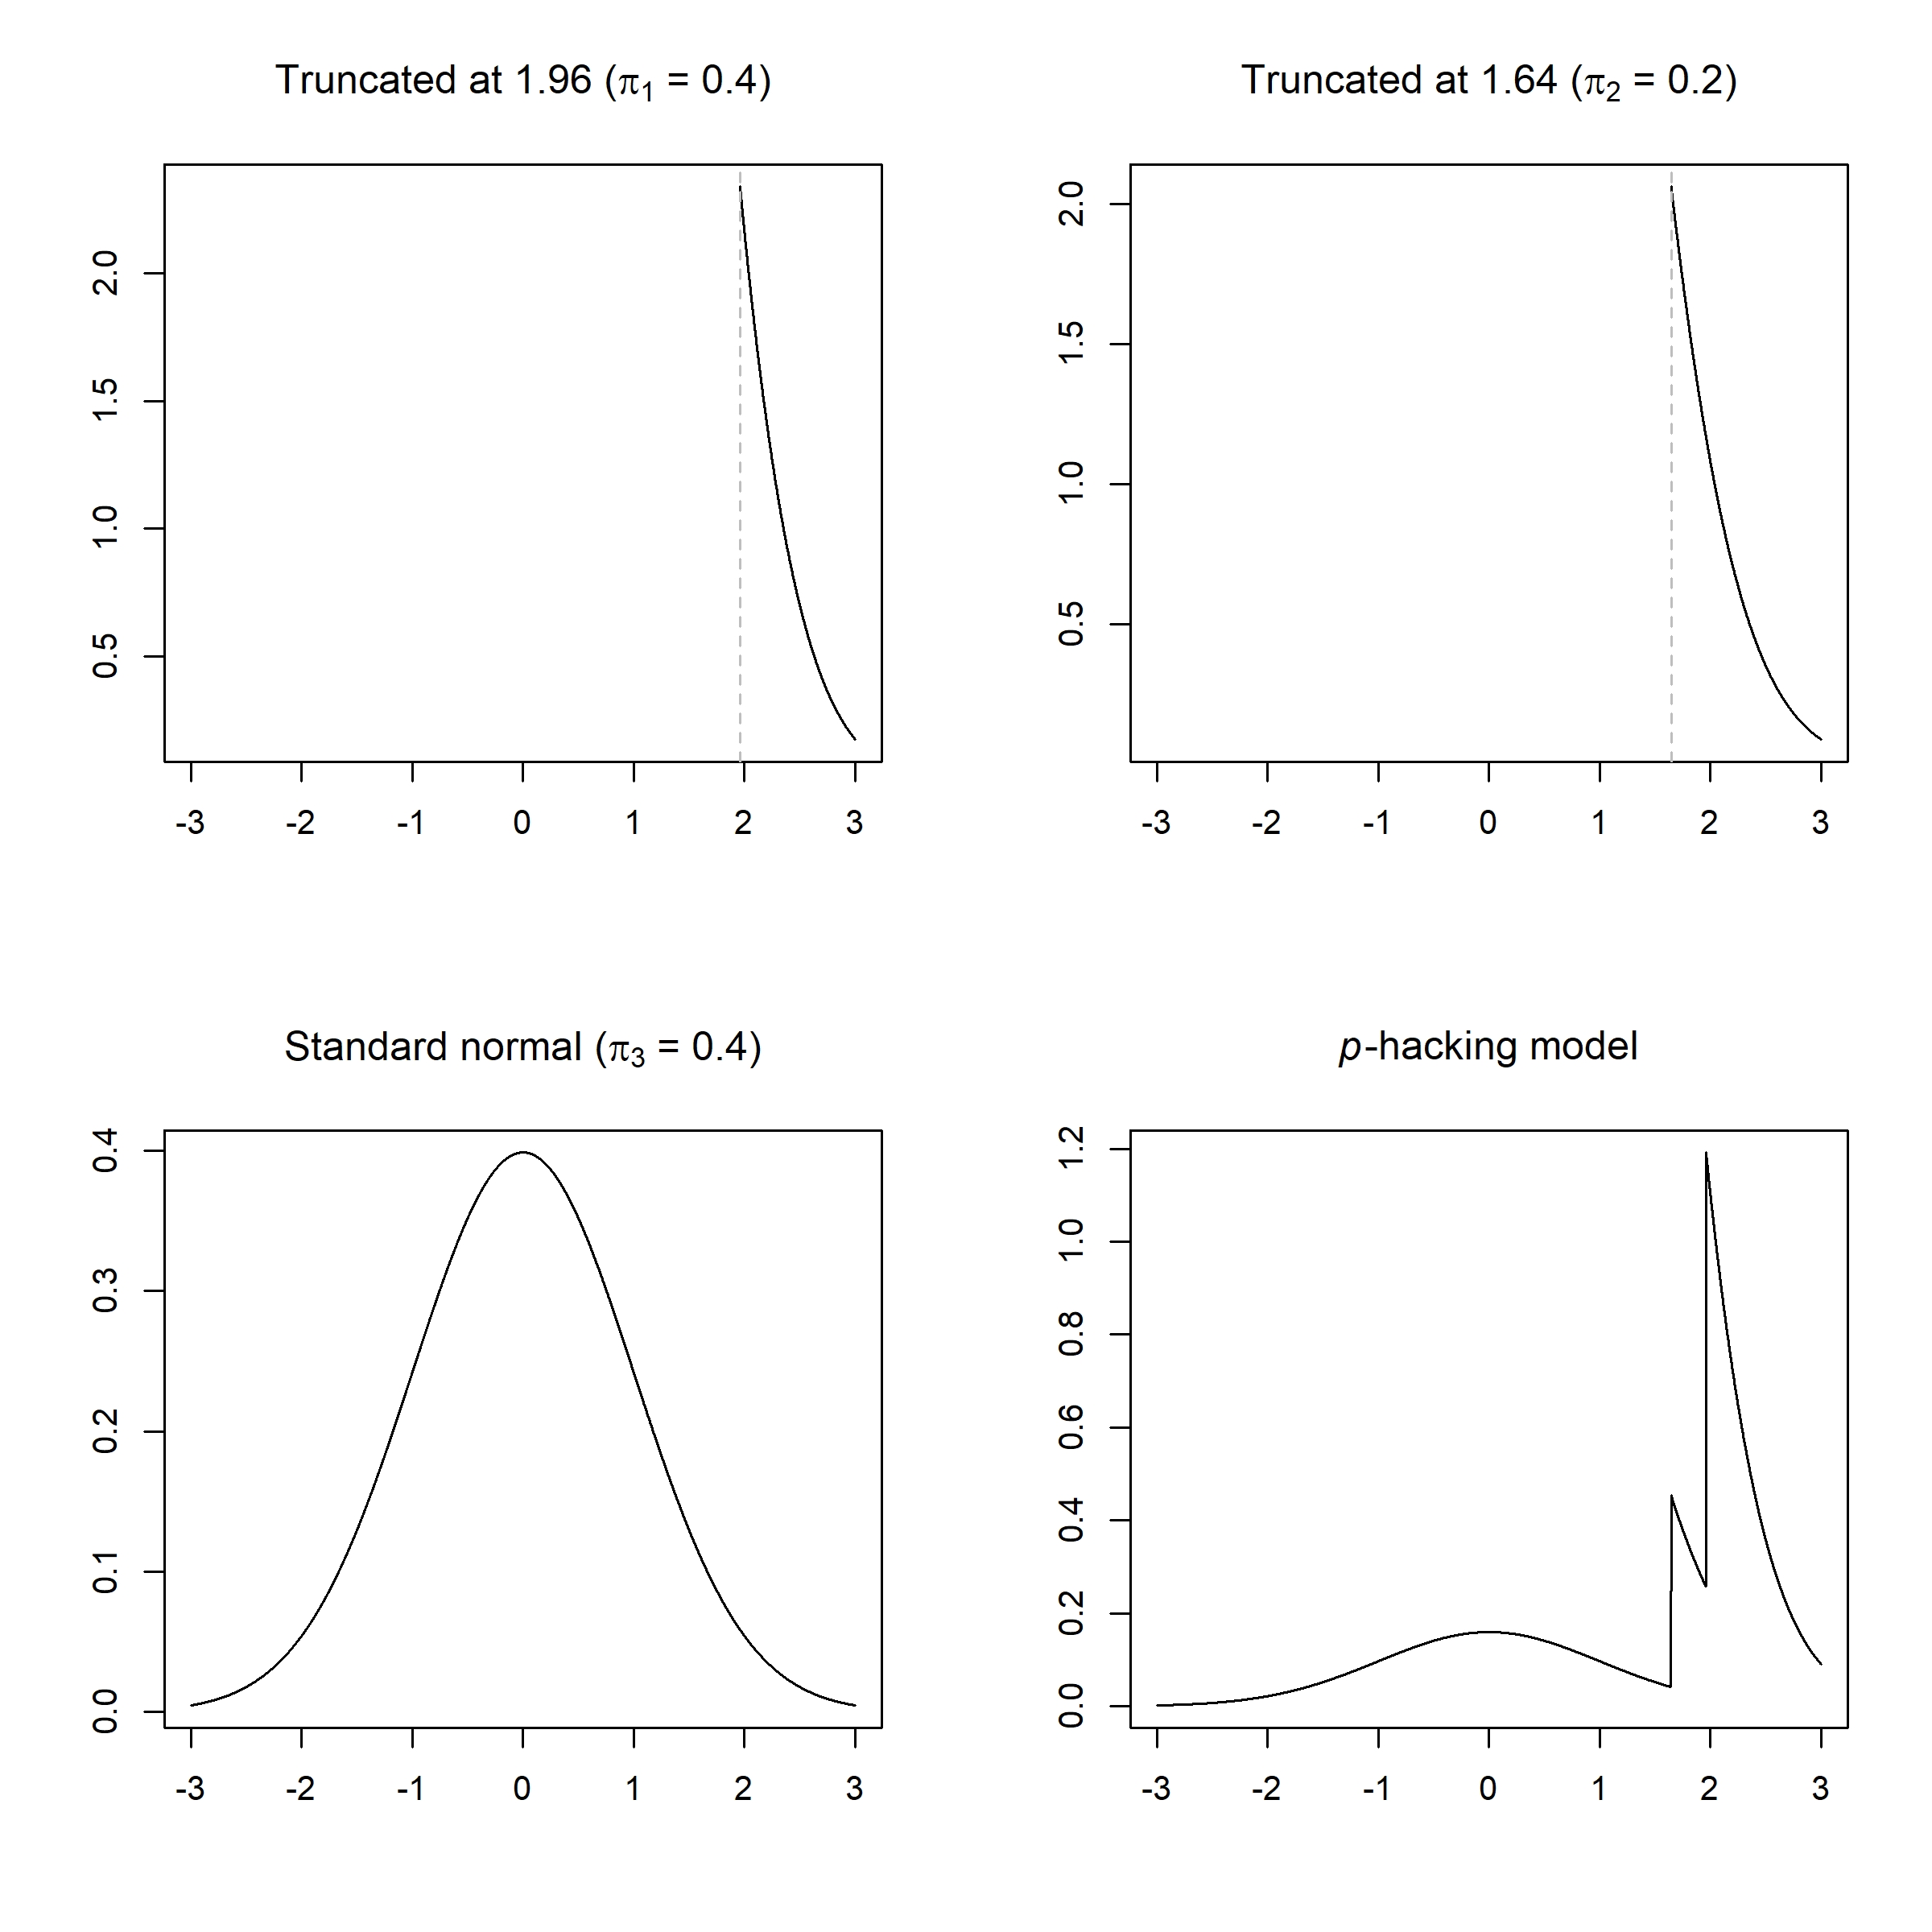
\includegraphics[scale=0.5]{plots/p-hacking}
\par\end{centering}
\caption{\label{fig:p-hacking plots}Illustration of the mixture components
of the \emph{p-}hacking model.}

\end{figure}

The publication bias model and the \emph{p}-hacking models are equivalent
under the fixed effects meta-analysis model, as formalized by the
following Lemma.
\begin{lem}
\label{lem:equivalence}Let $\{\sigma_{i}\}_{i=1}^{n}$ be
a collection of standard deviations and $\theta\in\mathbb{R}$ be
an underlying mean. Then there is a bijective function $g(\pi)=\pi^{\star}$
so that $\prod f_{\textrm{ph}}(x_{i}\mid\theta,\sigma_{i},\pi)=\prod f_{\textrm{pb}}(x_{i}\mid\theta,\sigma_{i},g(\pi))$
for any collection $\{x_{i}\}_{i=1}^{n}$ of observations.
\end{lem}

\begin{proof}
It suffices to show there is a bijective function function $g(\pi)=\pi^{\star}$
so that $f_{\textrm{ph}}(x_{i}\mid\theta,\sigma_{i},\pi)=f_{\textrm{pb}}(x_{i}\mid\theta,\sigma_{i},g(\pi))$
that is independent of $\sigma_{i}$. To do this, define $g(\pi)$
by $\pi_{j}^{\star}=a_{j}^{\star}\sum_{i=j}^{J}\frac{\pi_{j}}{a_{j}}$
to make a bijective function between $\pi$ and $\pi^{\star}$. Now
observe that both $a_{j}^{\star}$ and $a_{j}$ are independent of
$\sigma_{i}$ when $\theta$ is fixed. Thus $g(\pi)$ is independent
of $\sigma_{i}$ and the proof is done.
\end{proof}
You may use this lemma to transform the $\pi$s on the \emph{p}-hacking
form into $\pi^{\star}$ on the publication bias form and vice versa. 
\bibliographystyle{biom}
\bibliography{edited.bib}

\end{document}